\documentclass{article}

\usepackage{tabto}
\usepackage{graphicx}

\begin{document}
\title{\LARGE Assignment 3}
\author{Jianqiang Du\\\\017547307}
\maketitle

\section{Exercise 3.25 (last question)}
\begin{itemize}
\item[Q:]The \textbf{heuristic path algorithm} (Pohl, 1977) is a best-first search in which the evaluation function is \textit f(\textit n) = (2 - \textit w)\textit g(\textit n) + \textit{wh}(\textit n). What kind of search does this perform for \textit w = 0, \textit w = 1, and \textit w = 2?
\item[A:]
\begin{itemize}
\setlength{\itemindent}{0.2in}
\item[\textit w = 0:]Uniform Cost Search
\item[\textit w = 1:]A* Search
\item[\textit w = 2:]Greedy Best First Search
\end{itemize}
\end{itemize}

\section{Exercise 4.1: (a) and (d)}
\begin{itemize}
\item[Q:]Give the name of the algorithm that results from each of the following special cases:
\begin{itemize}
\item[a.]Local beam search with \textit k = 1.
\item[d.]Simulated annealing with \textit T = $\infty$ at all times.
\end{itemize}
\begin{itemize}
\setlength{\itemindent}{-0.3in}
\item[A:]
\begin{itemize}
\setlength{\itemindent}{-0.07in}
\item[a.]Hill climbing search.
\setlength{\itemindent}{-0.37in}
\item[d.]Random walk
\end{itemize}
\end{itemize}
\end{itemize}

\section{Exercise 5.3: (a), (b), and (c)}
\begin{itemize}
\item[Q:]Imagine that, in Exercise 3.3, one of the friends wants to avoid the other. The problem then becomes a two-player \textbf{pursuit-evasion} game. We assume now that the players take turns moving. The game ends only when the players are on the same node; the terminal payoff to the pursuer is minus the total time taken. (The evader ``wins'' by never losing.) An example is shown in Figure 5.16.
\begin{itemize}
\item[a.]Copy the game tree and mark the values of the terminal nodes.
\item[b.]Next to each internal node, write the strongest fact you can infer about its value (a number, one or more inequalities such as ``$\geq$ 14", or a ``?").
\item[c.]Beneath each question mark, write the name of the node reached by that branch.
\end{itemize}

\begin{figure}[h!]
\centering
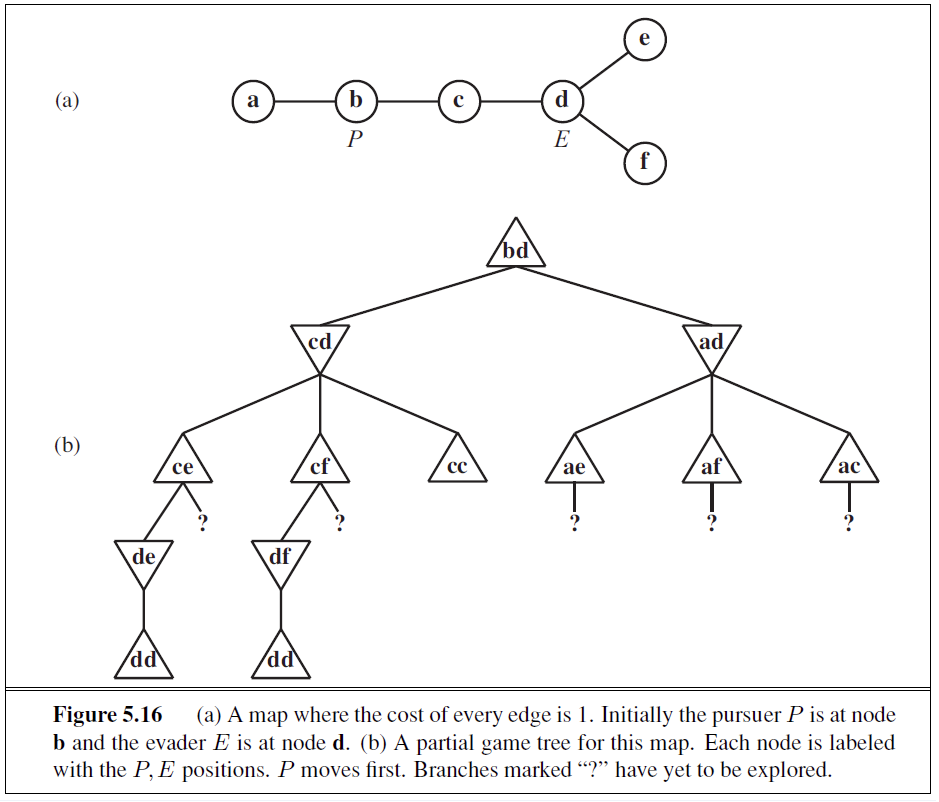
\includegraphics[width=0.8\textwidth]{fig5_16.png}
\end{figure}

\hspace*{-1em}A:\\
\begin{figure}[h!]
\centering
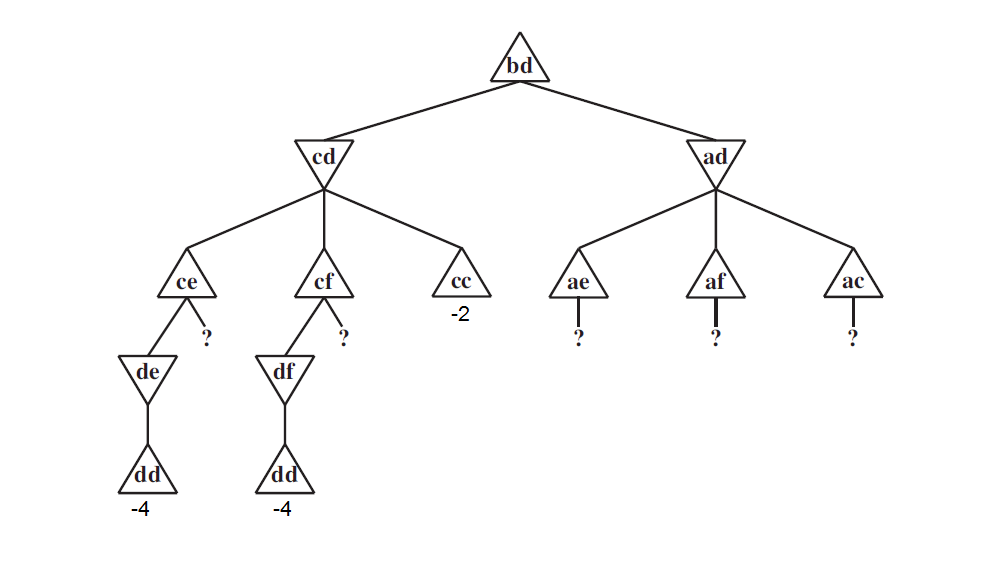
\includegraphics[width=\textwidth]{fig5_16(a).png}
\title{a.}
\end{figure}
\begin{figure}[h!]
\centering
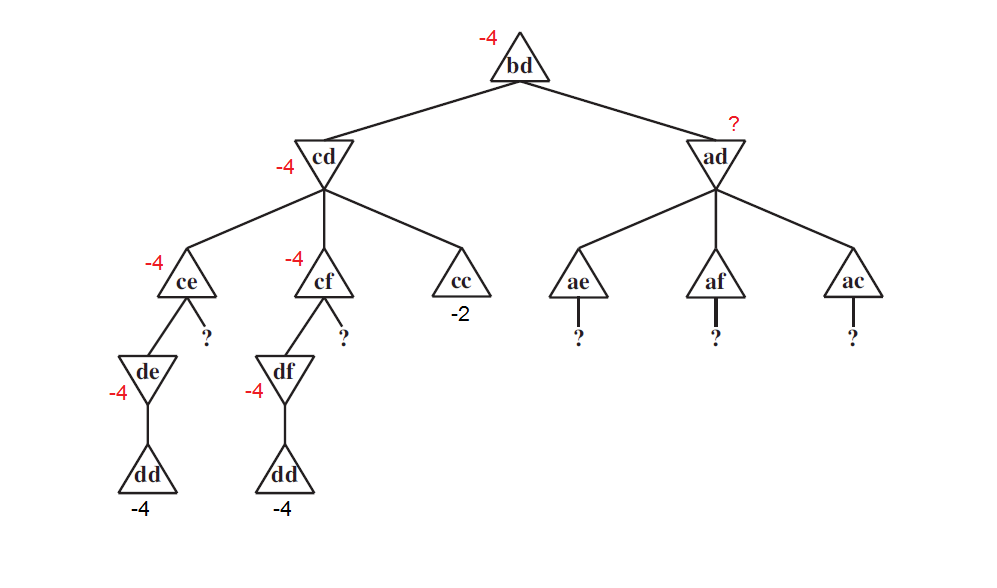
\includegraphics[width=\textwidth]{fig5_16(b).png}
\title{b.}
\end{figure}
\begin{figure}[h!]
\centering
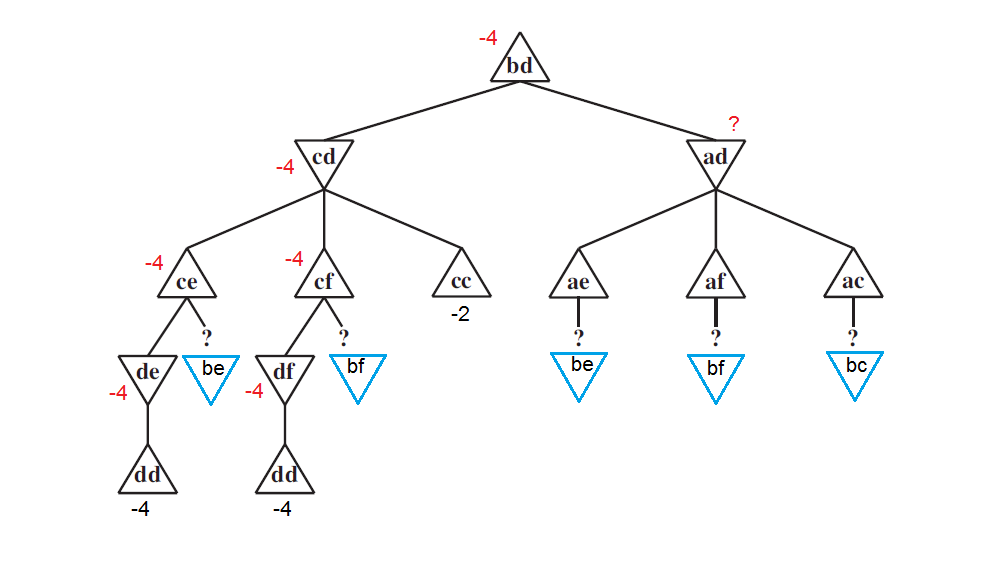
\includegraphics[width=\textwidth]{fig5_16(c).png}
\title{c.}
\end{figure}
\end{itemize}
\end{document}